\chapter{Análisis}\label{chap:Analisis}
En el capítulo anterior se listaron distintas tecnologías que podían sernos útiles para nuestro proyecto. En el actual nos detendremos a explicar cuáles de ellas explicaremos y el por qué de su elección.

\section{Simulador de redes: GNS3}
Se ha decidido que GNS3 sea el simulador de redes a utilizar para nuestro proyecto por varias razones:
\begin{itemize}
\item Es \textbf{multiplataforma}, con lo que podemos trabajar sencillamente con él tanto desde Windows como Linux.
\item Existe \textbf{mucha información} para consultar. Desde internet contamos con documentación oficial y un foro propio. Hay incluso libros sobre él y como ejemplo tenemos el usado en varias ocasiones en este documento, ``The Book of GNS3'', por Jason C. Neumann.
\item Es altamente \textbf{expandible}: hay decenas de aparatos reales que pueden incluirse y emularse en las topologías creadas. Pueden descargarse desde \MYhref{https://www.gns3.com/marketplace/appliances}{su marketplace}.
\item \textbf{Cuenta con una API REST} que lo hace interactivo desde el exterior.
\item Integra \textbf{WireShark} nativamente para estudiar el envío de datos entre los distintos dispositivos.
\end{itemize}

Con la descripción de simulador y emulador de red que pudo verse en la sección \ref{sec:simuladoremulador}, entendemos que GNS3 es un simulador (tal y como es descrito en la mayoría de fuentes) que incluye en sí mismo una serie de emuladores que ayudan a recrear los entornos. Las emulaciones son posibles gracias a herramientas como QEMU (un emulador de máquinas y virtualizador open source \cite{qemu}). Lo que ocurre entre los distintos dispositivos (emulados) desplegados en GNS3 es lo que el software simula.

GNS3 se estructura en \textbf{proyectos}. En cada proyecto podemos desplegar una serie de dispositivos y conectarlos entre sí. Al guardar un proyecto como tal, el despliegue realizado se guarda junto a él. Sin embargo, el estado de las máquinas no corre la misma suerte, y es que a cada apagado de las mismas toda su configuración se pierde.

Una de las características más interesantes de GNS3 y sus proyectos está en la importación y exportación de estos. El simulador cuenta con una opción que permite extraer todo un proyecto en una imagen (de formato \textit{.gns3project}) para que sea fácilmente portable. Existe la posibilidad de exportar, junto a la topología creada, las imágenes base sobre las que los nodos del proyecto están construidas para que no sea necesario contar con esas imágenes en el GNS3 donde se pretende importar.

\begin{figure}[h]
  \centering
  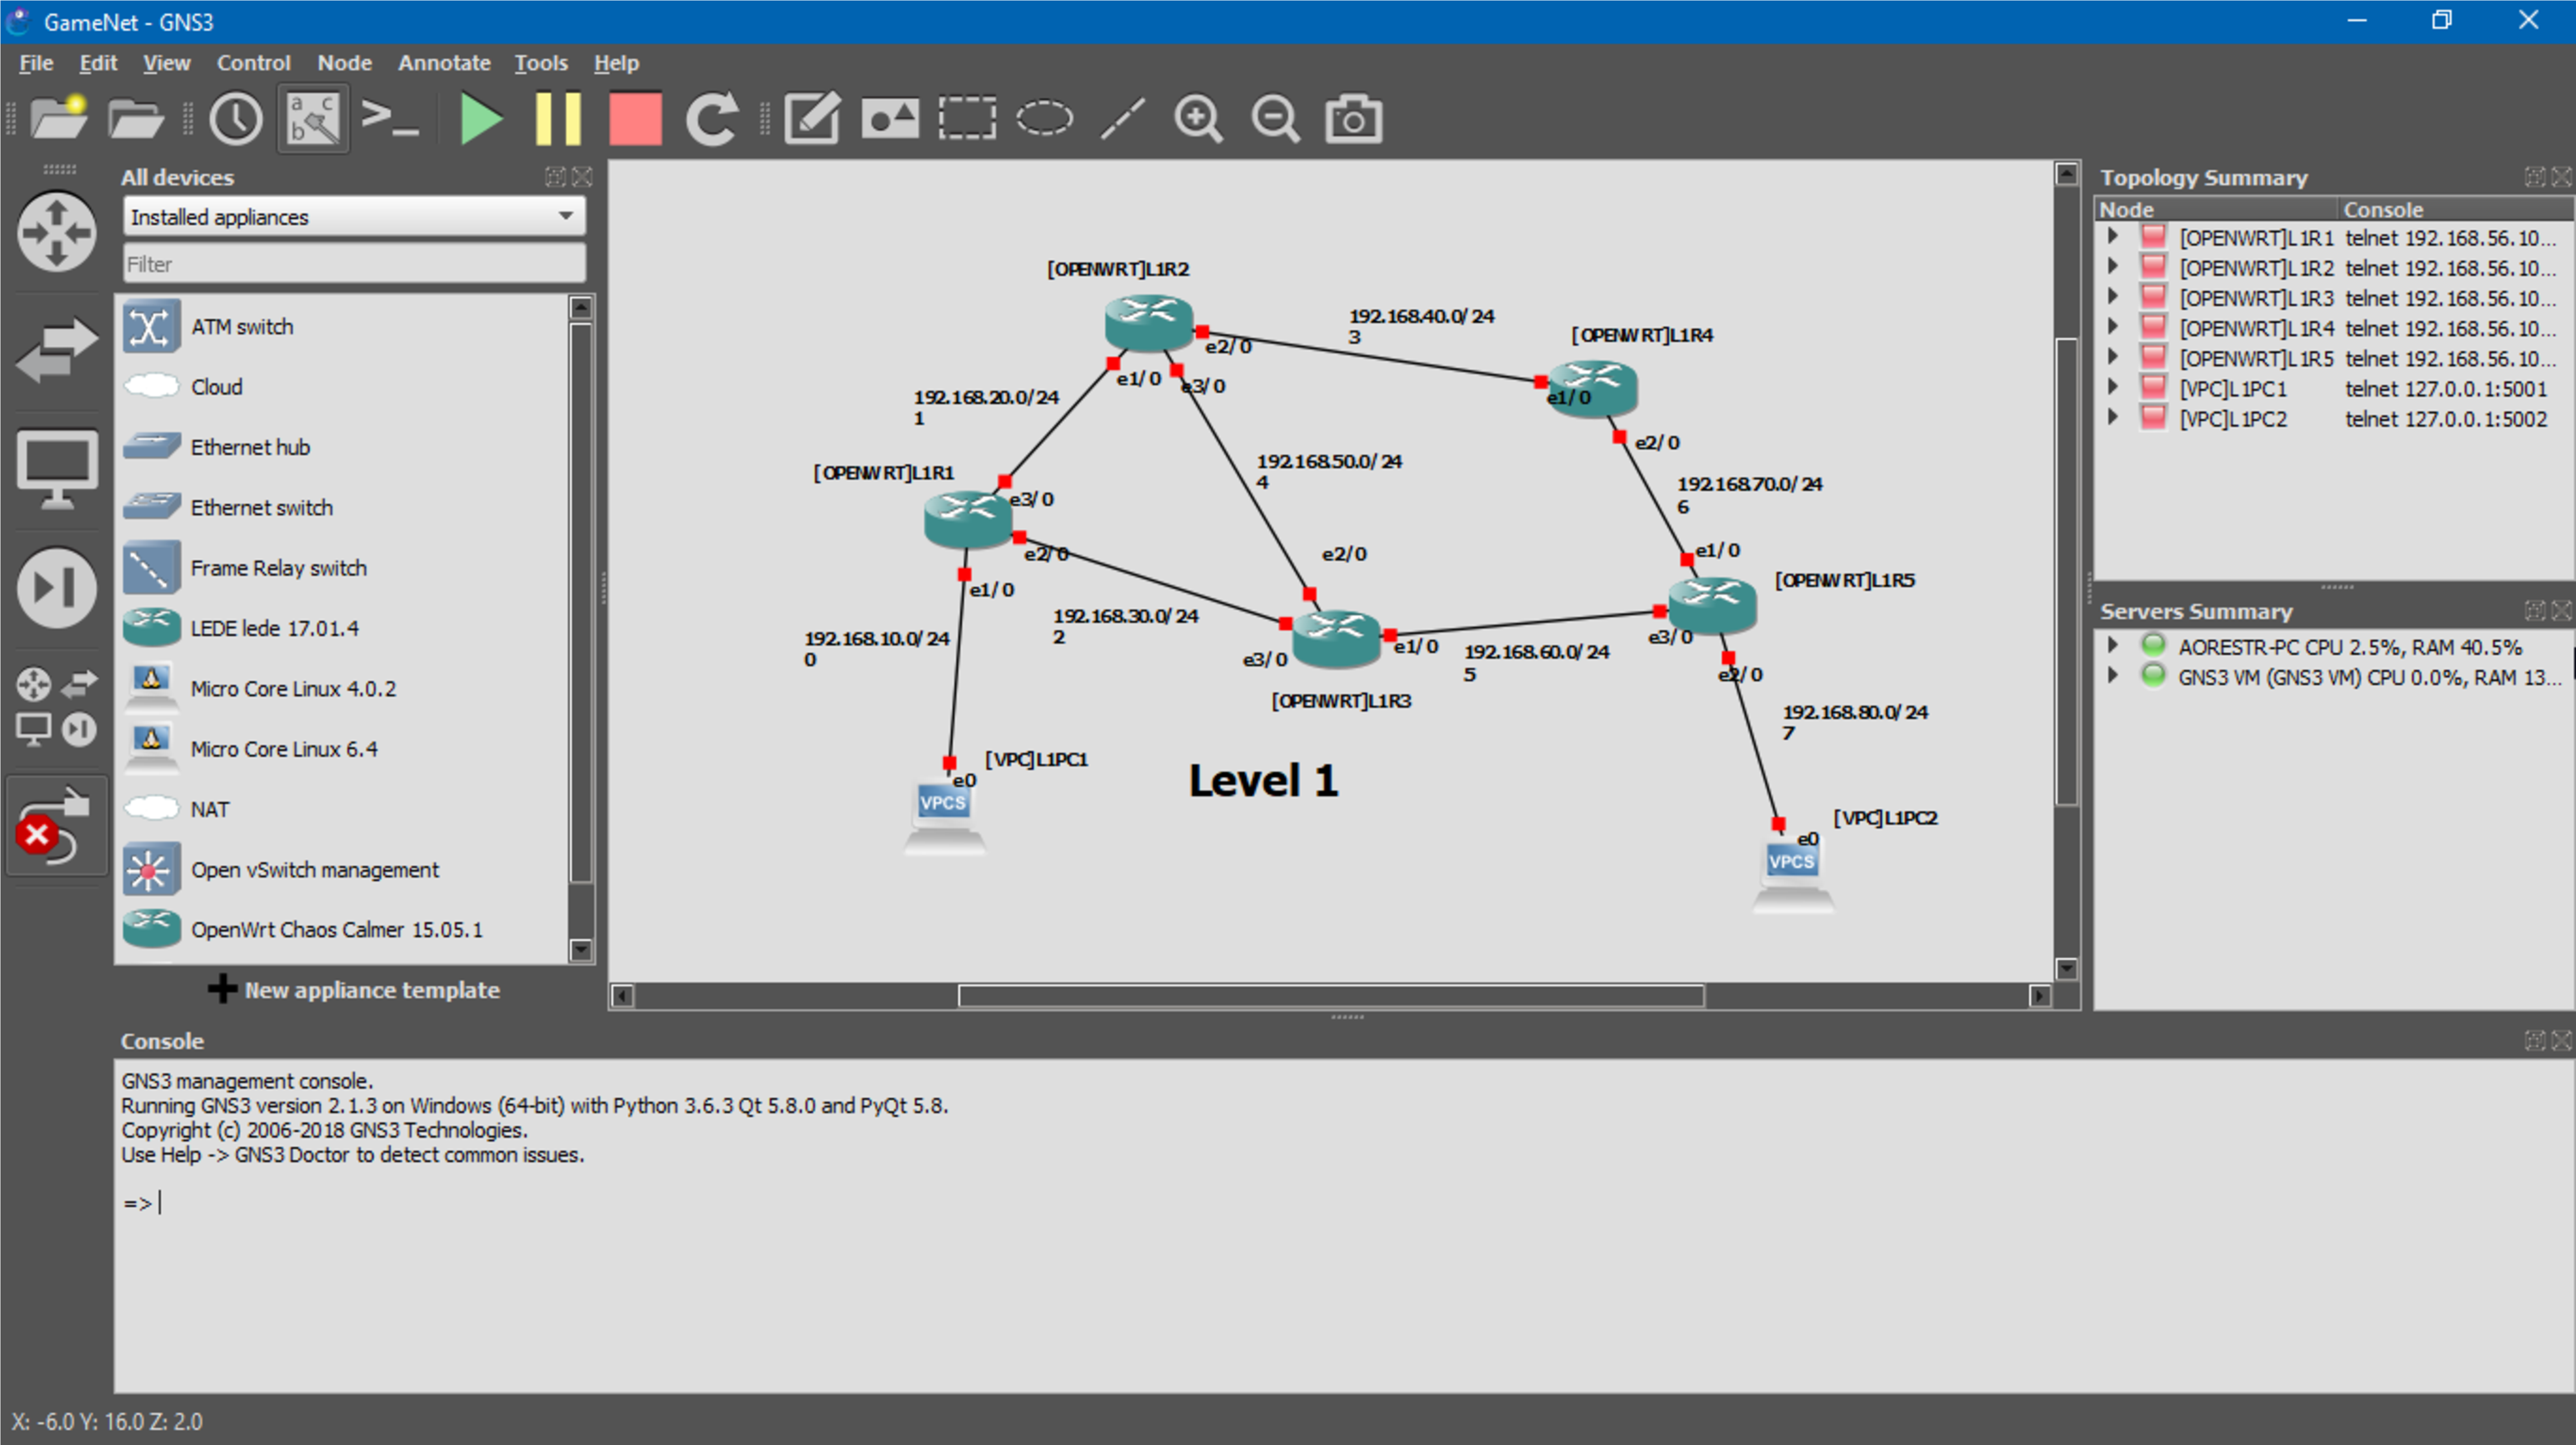
\includegraphics[scale=0.15]{imagenes/interfazgns}
  \caption{Interfaz de GNS3}
  \label{fig:interfazgns}
\end{figure}

La interfaz de usuario de la aplicación puede verse en la figura \ref{fig:interfazgns}. La barra de arriba está repleta de opciones relacionadas con el proyecto, como arrancar todos los dispositivos, pausarlos, pararlos o incluso herramientas de dibujo para convertir el esquema en algo más intuitivo y legible. A la izquierda se listan los nodos disponibles en la máquina. Arrastrándolos al centro los insertamos en el proyecto.

A continuación pasaremos a explicar conceptos clave del emulador.

\subsection{Arquitectura de GNS3}
La documentación de GNS3 recoge el modo en el que la aplicación está estructurada. La ilustración \ref{fig:estructuragns3} está sacada directamente de ella \cite{structuregns3}.

\begin{figure}[h]
  \centering
  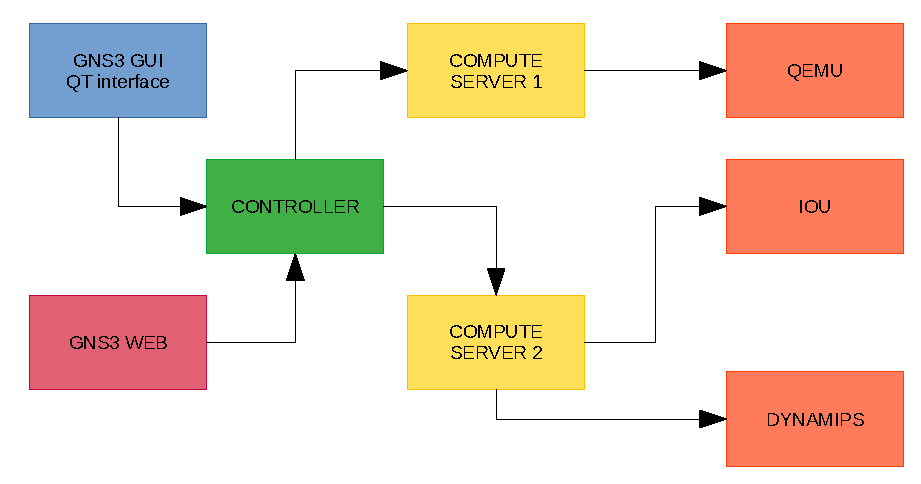
\includegraphics[scale=0.6]{imagenes/estructuragns3}
  \caption{Estructura interna de GNS3}
  \label{fig:estructuragns3}
\end{figure}

Las distintas partes que componen la aplicación se transmiten la información sobre HTTP haciendo uso de mensajes JSON (del inglés, \textit{JavaScript Object Notation}), un formato de intercambio de datos ligero fácil de leer y escribir para humanos \cite{JSON}.

Volviendo a la imagen, el controlador (\textit{controller}) controla todo la parte que gestiona el estado de un proyecto y lo guarda en el disco. Sólo existe un controlador para toda la aplicación. El GUI o interfaz de usuario es la encargada de mostrar las topologías. Toda la información que necesita la toma directamente del controlador. En los ``compute'' es donde se ejecutan los emuladores. Para cada aparato de la topología se inicia una instancia de emulador.

\subsection{El servidor}
El controlador y los ``compute'' de GNS3 forman el servidor del mismo. GNS3 aprovecha la tecnología cliente-servidor; al igual que un navegador web se conecta a un servidor web para acceder a las páginas web y mostrarlas, el GUI accede al servidor, permitiendo que se inicie, pare y controlar los dispositivos desplegados. Esto permite que los proyectos sean fácilmente escalables, ya que no necesitan ser ejecutados en un único equipo. Si se pretende trabajar con topologías grandes o complejas, también se puede ejecutar el servidor GNS3 en un PC diferente a aquel donde el GUI es ejecutado. Por consiguiente, de contar con un servidor de altas prestaciones, es posible instalar el servidor de GNS3 allí y desde otro sistema remoto construir y controlar las redes \cite{bookgns}.

\subsection{La API}
GNS3 habilita la interacción con el servidor mediante una API REST (cuyo significado será explicado en la sección \ref{subsec:sectionapi}). Mediante el protocolo de red HTTP es posible construir proyectos y llenarlos con nodos y enlaces (que se definirán a continuación) sin necesidad de hacer uso de la interfaz de usuario. En la breve \MYhref{https://gns3-server.readthedocs.io/en/latest/curl.html}{documentación de la API} oficial es posible ver algunos ejemplos de uso.

GNS3 se encarga de asignar a cada proyecto un ID único. Un ejemplo de recurso puede ser el siguiente, donde se accede a un JSON con los proyectos abiertos en GNS3 e información básica sobre ellos: \textit{http://$<$IP del server$>$:$<$puerto del servidor$>$/v2/projects}.

\subsection{Nodos}
Cada dispositivo de una red está representado en GNS3 por un elemento llamado \textbf{nodo}. Estos nodos, que pueden ser desde un router a un switch, no son más que virtualizaciones de aparatos reales. Por norma general, las virtualizaciones se realizan a partir de imágenes de los sistemas operativos que se integran en los aparatos. Así, podemos tener varios routers distintos de Cisco montados sobre la misma estructura, permitiéndonos jugar con ellos con verdadera facilidad.

Tanto en macOS como en Windows es necesario utilizar \textbf{GNS3 VM} para hacer uso de ciertos nodos. Se trata de una imagen con un Ubuntu ligero que se instala en un hipervisor (VMware, Virtualbox) y hace de sistema operativo desde el que ejecutar los aparatos que se implanten en la red. Las ventajas de usar GNS3 VM son las siguientes \cite{gns3vm}:
\begin{itemize}
\item Algunas dependencias son difíciles de instalar, como los requisitos para IOU; necesitan una librería específica.
\item Con VMware es posible utilizar utilizar la aceleración KVM para QEMU.
\item Dynamips y QEMU funcionan mejor en Linux (menos problemas aleatorios con ASA por ejemplo).
\item Soporte completo de IOU.
\item No hay antivirus o firewall dentro de la máquina virtual que modifique el tráfico de la red.
\item La máquina está aislada del host, lo que implica un mayor nivel de seguridad.
\end{itemize}

Los nodos pueden ser inicializados juntos (todos los del proyecto a la vez) o por separado. GNS3 los asigna a un puerto de la red desde el que pueden ser accedidos y controlados mediante telnet.

En la API, para obtener los distintos nodos que existen un proyecto es necesario acceder al recurso: \textit{http://$<$IP del server$>$:$<$puerto del servidor$>$/v2/projects/$<$ID del proyecto$>$/nodes}

\subsection{Enlaces}
Los nodos están interconectados entre sí mediante enlaces. Los enlaces son los encargados del envío de paquetes entre ellos. Sus características pueden ser modificados mediante ``filtros de paquete'' (\textit{Packet filters}), que no son más que unos parámetros que afectan a las conexiones. Desde la latencia a la probabilidad de pérdida de paquetes se puede controlar mediante ellos.

El recurso asociado en la API a los enlaces de un proyecto es: \textit{http://$<$IP del server$>$:$<$puerto del servidor$>$/v2/projects/$<$ID del proyecto$>$/links}
 
\section{Motor de videojuegos: Unity}
\subsection{Ventajas sobre otros motores}
Una de las principales razones por las que se ha elegido Unity como el motor sobre el que desarrollar nuestro juego es por su popularidad y su facilidad de aprendizaje. Cuenta con toneladas de información en la red y con foros muy activos que permiten encontrar respuesta a las preguntas generadas a gran velocidad. Pero Unity es una buena elección también por méritos propios.

El motor posee simulación física propia, oclusión ambiental (SSAO), sombras dinámicas... y una larga lista de elementos más. Muchos motores de juego cuentan también de estas características, pero Unity tiene dos ventajas principales sobre otras herramientas de desarrollo de juegos igualmente avanzadas: un flujo de trabajo visual (\textit{visual workflow}) extremadamente productivo y un alto grado de compatibilidad entre plataformas.

El workflow visual posee un diseño bastante único, diferente de la mayoría de los otros entornos. El editor se utiliza para diseñar las escenas de su juego y para unir los ``assets'' (cuyo significado veremos más adelante) de arte y el código en objetos interactivos. Lo bueno de este editor es que permite crear juegos de calidad profesional de forma rápida y eficaz, proporcionando a los desarrolladores herramientas increíblemente productivas a la vez que utilizando las últimas tecnologías en el mundo de los videojuegos.

El editor es especialmente útil para hacer iteraciones rápidas, permitiendo perfeccionar el juego a través de ciclos de protipado y pruebas. Se pueden ajustar objetos en el editor y mover cosas incluso mientras el juego está en marcha. Además, Unity permite personalizar el editor mismo escribiendo scripts que añaden nuevas funciones y menús a la interfaz.

Además de las importantes ventajas en cuanto a productividad del editor, el otro punto fuerte del conjunto de herramientas de Unity es el alto grado de compatibilidad entre plataformas. Unity no sólo es multiplataforma en cuanto a los objetivos de implementación (se puede implementar en el PC, la web, el móvil o las consolas), sino que es multiplataforma en cuanto a las herramientas de desarrollo (se puede desarrollar el juego en Windows o macOS). Esta naturaleza se debe en gran medida a que Unity comenzó como software sólo para Mac y más tarde fue portado a Windows. La primera versión fue lanzada en 2005. Actualmente se encuentra en su quinta versión principal (con muchas actualizaciones menores que se publican con frecuencia). Inicialmente, Unity sólo soportaba Mac tanto para el desarrollo como para la implementación, pero en pocos meses Unity se había actualizado para funcionar también en Windows.

Mientras tanto, el sistema de componentes modulares utilizado para construir objetos de juego aporta un tercer y más sutil beneficio. En un sistema de componentes, los "componentes" son paquetes de funcionalidad de mezcla y correspondencia, y los objetos son construido como un conjunto de componentes más que como una estricta jerarquía de clases. En otras palabras, un sistema de componentes es un enfoque diferente (y generalmente más flexible) a la hora de hacer programación orientada a objetos, donde los objetos del juego se construyen a través de composición en lugar de herencia.

En un sistema de componentes, los objetos existen en una jerarquía plana y diferentes objetos tienen diferentes colecciones de componentes. Esto difiere de una estructura de herencia, donde diferentes objetos se encuentran en ramas completamente diferentes del árbol. Esta disposición facilita la creación rápida de prototipos, ya que puede mezclar y combinar rápidamente diferentes componentes en lugar de tener que refactorizar la cadena de herencia cuando los objetos cambian.

Aunque podría escribirse código para implementar un sistema de componentes personalizado si no existiera, Unity ya tiene un sistema de componentes robusto; sistema integrado perfectamente con el editor visual. En lugar de manipular componentes en código, es posible adjuntar y separar componentes dentro del editor visual. No se está limitado a construir sólo objetos a través de la composición: existe además la opción de usar herencia en el propio código.

\subsection{Desventajas}
Unity tiene muchas ventajas que la convierten en una gran elección para el desarrollo de juegos pero, como cualquier otra herramienta, tiene sus puntos débiles. En particular, la combinación del editor visual y un código muy elaborado por debajo, aunque muy efectiva con el sistema de componentes de Unity, es inusual y puede crear dificultades. En escenas complejas, puede perderse la pista de qué objetos de la escena tienen componentes específicos. Unity proporciona funcionalidades de búsqueda para encontrar scripts adjuntos, pero esa búsqueda quizás debería ser más robusta; a día de hoy es posible encontrar situaciones en las que es necesario inspeccionar manualmente todo lo que hay en la escena para encontrar vínculos de scripts.

Una otra desventanja tiene que ver con el trabajo con ``prefabs''. Los prefabs son un concepto específico de Unity. Se trata de un enfoque flexible para definir visualmente los objetos interactivos. El concepto de prefab es poderoso y único, pero puede llegar a ser especialmente incómodo el editar prefabs. Considerando que son una parte útil y central del trabajo con Unity, se espera que las versiones futuras mejoren el flujo de trabajo para su edición.

\subsection{Interfaz de usuario}
La figura mostrada a continuación ilustra un ejemplo de la interfaz de usuario del motor.

\begin{figure}[H]
  \centering
  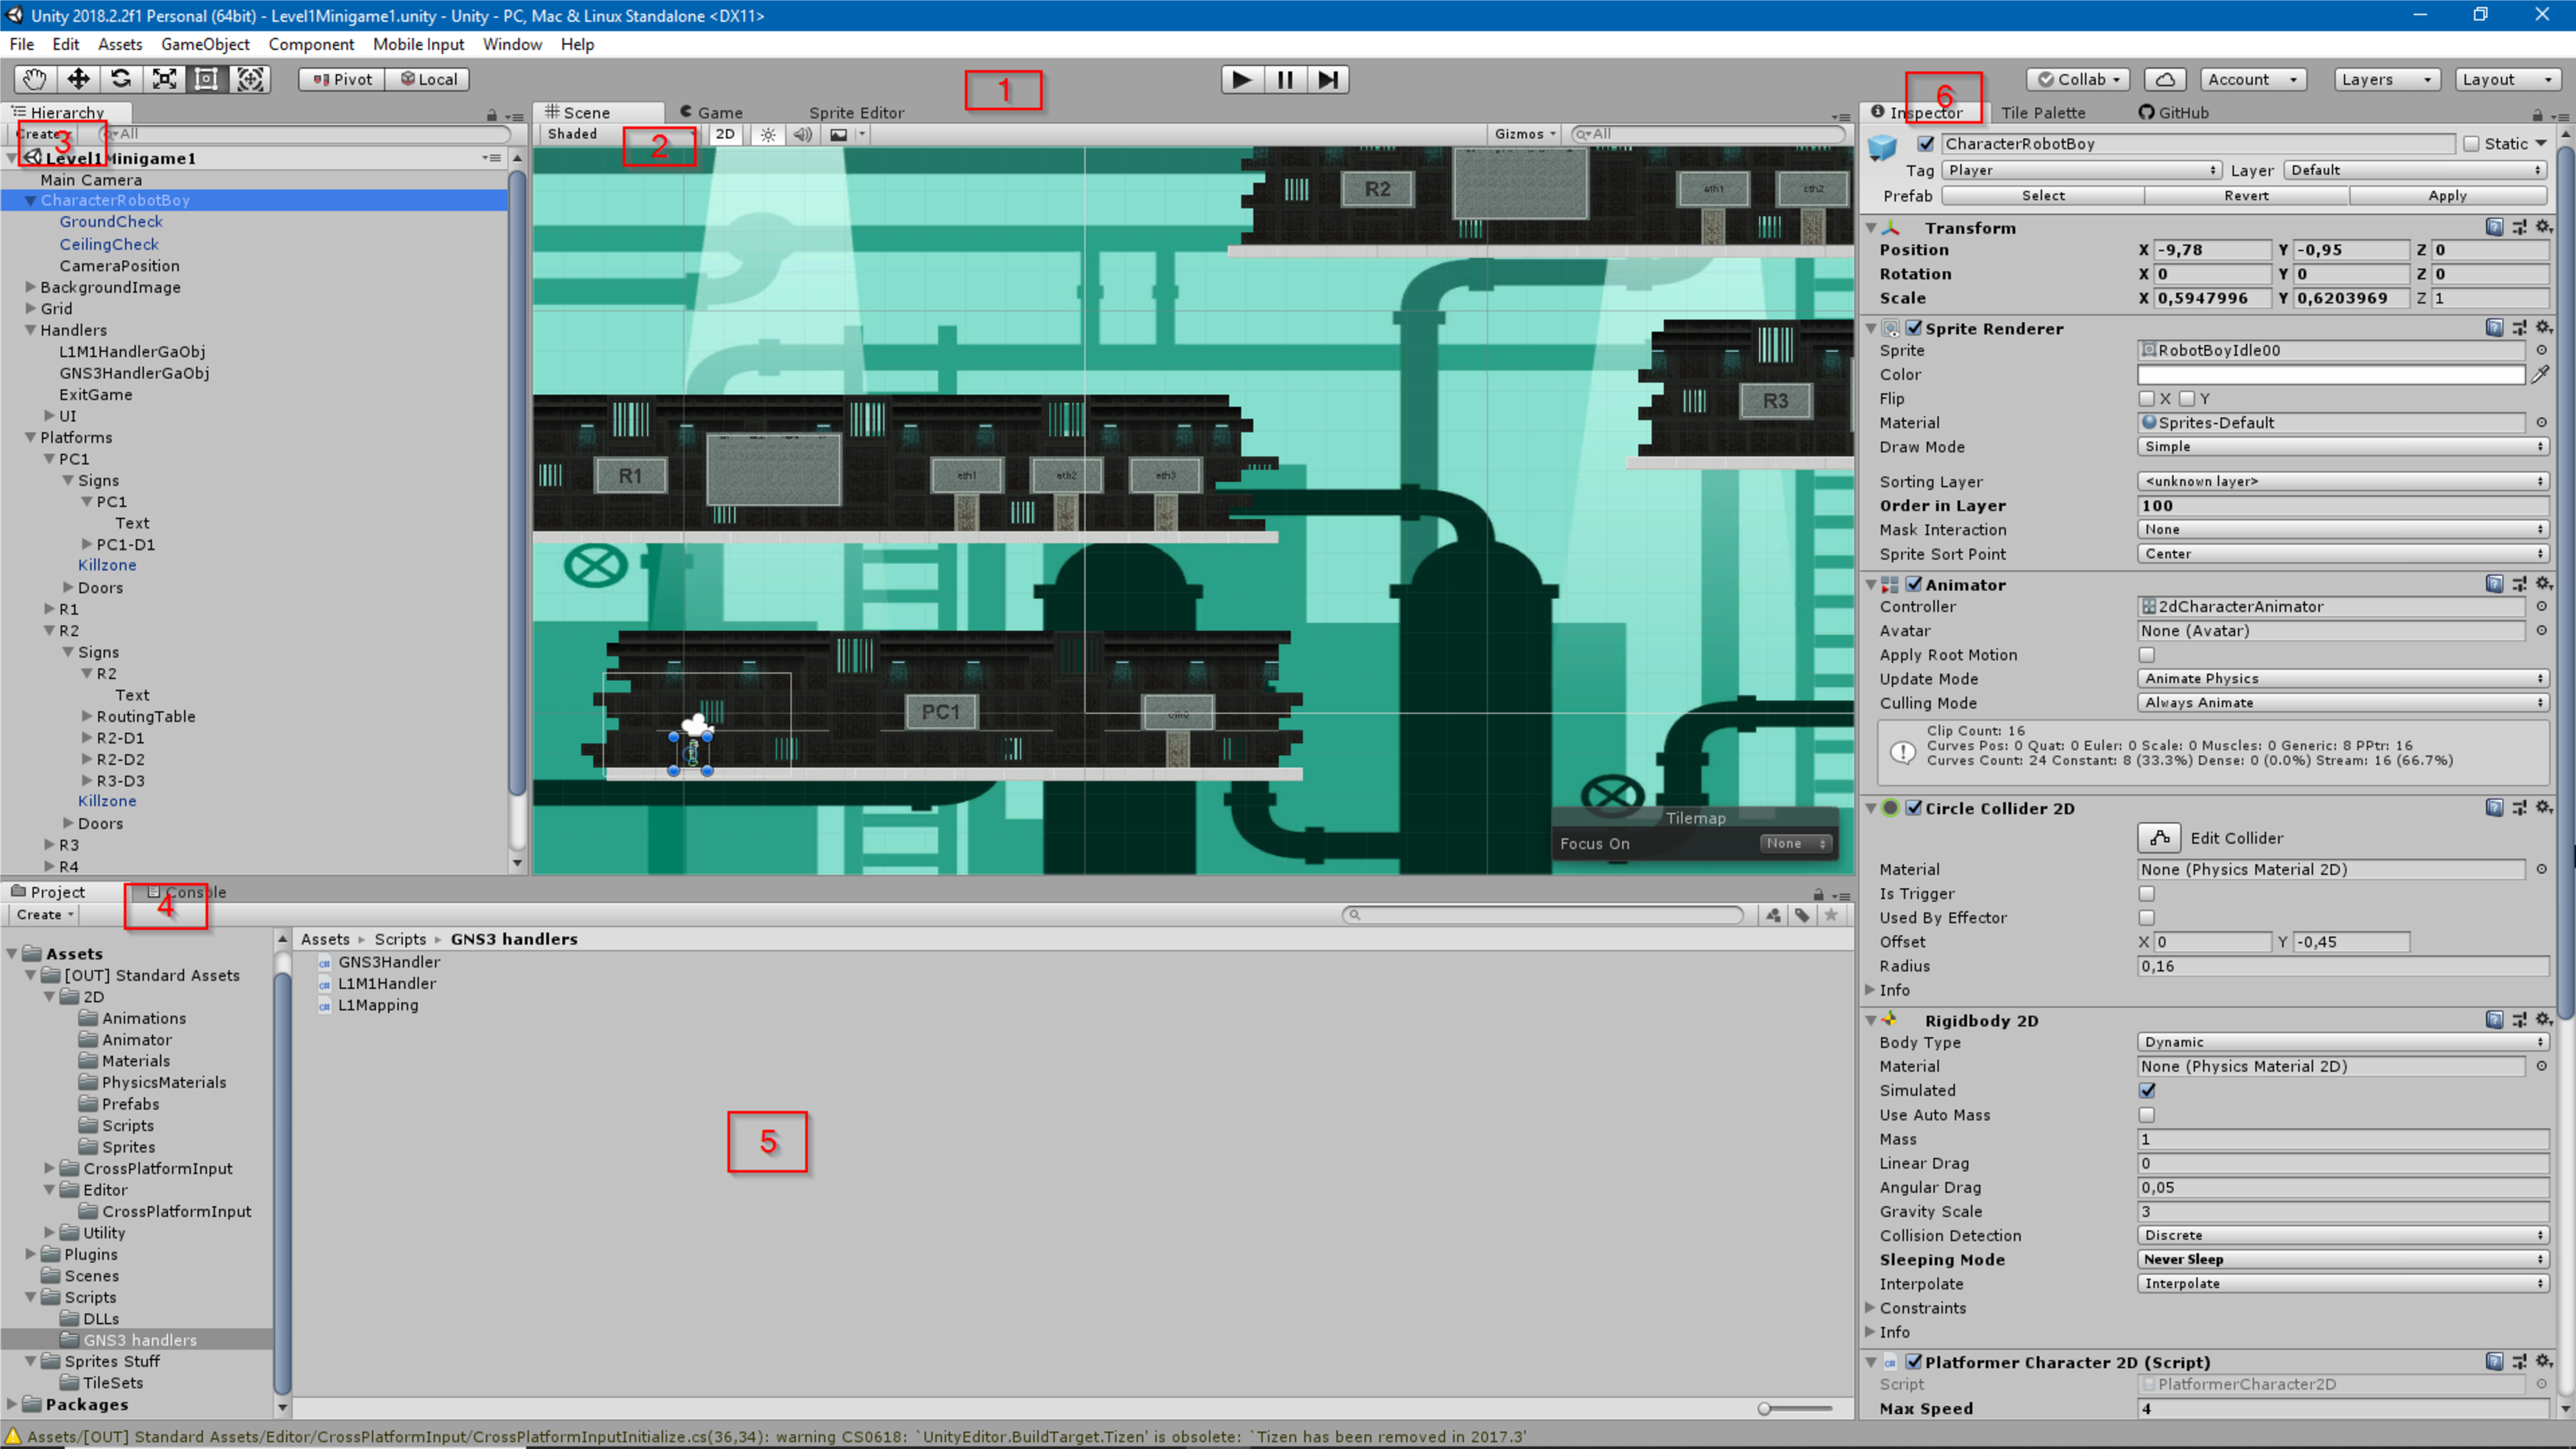
\includegraphics[scale=0.11]{imagenes/uiunity}
  \caption{Interfaz de usuario de Unity}
  \label{fig:uiunity}
\end{figure} 

\begin{enumerate}
\item Toda el área superior es la barra de herramientas. A la izquierda hay botones para desplazar la vista de la escena y mover objetos de la misma, y en el centro está el botón arranque para lanzar la escena que esté siendo editada.
\item ``Scene'' y ``Game'' son pestañas para ver la escena y jugar al juego, respectivamente.
\item ``Hierarchy'' muestra una lista de todos los objetos de la escena, anidados de acuerdo con la forma en que están vinculados entre sí. Con tan solo arrastrar objetos hacia esta pestaña es posible anidarlos entre sí.
\item ``Project'' y ``Console'' son pestañas para ver todos los archivos del proyecto y los mensajes del código, respectivamente.
\item Carpetas con los archivos relacionados con el proyecto.
\item El ``inspector'' ocupa todo el lado derecho. Muestra información sobre el objeto actualmente seleccionado (una lista de componentes). Estos componentes asociados al objeto son los que lo configuran y otorgan propiedades. Un script puede ser anclado como componente.
\end{enumerate}

A medida que el documento avance hablaremos de más herramientas y elementos de Unity que han sido necesarias para nuestro propósito.